%\documentclass[twoside]{pwrthesis}
\documentclass[twoside]{iisthesis}
% ---
\usepackage{polski}
\usepackage[utf8]{inputenc}
\usepackage{amsmath}
\usepackage{tocloft}
\usepackage{listings}
\usepackage{algorithm}
\usepackage{algorithmic}
\usepackage{subcaption}
\usepackage{mathtools}
\usepackage{graphicx}
\usepackage[colorinlistoftodos]{todonotes}
\usepackage{url}
\usepackage{pgfplots, pgfplotstable}
\selectlanguage{polish}
% Dodane przeze mnie d
\usepackage{fancyvrb} % dla srodowiska Verbatim
\usepackage{color}
\usepackage{lscape}

\hypersetup{
    colorlinks,
    linkcolor={black!50!black},
    citecolor={black!50!black},
    urlcolor={black!80!black}
}

\definecolor{gray}{rgb}{0.4,0.4,0.4}
\definecolor{darkblue}{rgb}{0.0,0.0,0.6}
\definecolor{cyan}{rgb}{0.0,0.6,0.6}

\lstset{
  basicstyle=\ttfamily,
  columns=fullflexible,
  showstringspaces=false,
  commentstyle=\color{gray}\upshape
}

\lstdefinelanguage{XML}
{
  morestring=[b]",
  morestring=[s]{>}{<},
  morecomment=[s]{<?}{?>},
  stringstyle=\color{black},
  identifierstyle=\color{darkblue},
  keywordstyle=\color{cyan},
  morekeywords={xmlns,version,type}% list your attributes here
}

\lstset{
  language=XML,
   literate={ć}{{\'c}}1
}
\renewcommand*{\lstlistingname}{Kod źródłowy}
% definicje kolorow
\definecolor{ciemnoSzary}{rgb}{0.15,0.15,0.15}
\definecolor{szary}{rgb}{0.5,0.5,0.5}
\definecolor{jasnoSzary}{rgb}{0.2,0.2,0.2}

% Konfiguracja verbatima
\fvset{
	frame=single,
	numbers=left,
	fontsize=\footnotesize,
	numbersep=12pt,
%	framerule=.5mm,
	rulecolor=\color{ciemnoSzary},
%	fillcolor=\color{jasnoSzary},
	framesep=4pt,
	stepnumber=1,
	numberblanklines=false,
	tabsize=2,
%	formatcom=\color{szary}
}
\newcommand{\listequationsname}{Spis wzorów}
\newcommand{\equationcaption}[1]{\begin{flushright}\emph{#1}\end{flushright}}
\newcommand{\rightcaption}[1]{\begin{flushright}\emph{#1}\end{flushright}}
\newlistof{myequations}{equ}{\listequationsname}
\newcommand{\myequations}[1]{%
\addcontentsline{equ}{myequations}{\protect\numberline{\theequation}#1}\par}

\newcommand{\listofmyalgorithmsname}{Spis algorytmów}
\newlistof{myalgorithm}{algo}{\listofmyalgorithmsname}
\newcommand{\myalgorithm}[1]{%
\addcontentsline{algo}{myalgorithm}{\protect\numberline{\thealgorithm}#1}\par}


\newcommand{\listofmyfiguresname}{Spis rysunków}
\newlistof{myfigure}{figu}{\listofmyfiguresname}
\newcommand{\myfigure}[1]{%
\addcontentsline{figu}{myfigure}{\protect\numberline{\thefigure}#1}\par}

\floatname{algorithm}{Algorytm}

\newtheorem{mydef}{Definicja}



\begin{document}


\newcommand{\resultChart}[7][140]{
\def\dataS{{#2}}
	\begin{figure}[H]
	
\centering

\begin{center}
\begin{tikzpicture}
 
\begin{axis}[
ybar,
bar width=20,
legend style={at={(0.5,-0.25)},
anchor=north,legend columns=-1},
ylabel={Wartość miary},
symbolic x coords={\dataS},
xtick=data,
height=  {#1},
width=0.8\textwidth,
ymin=0, ytick={0,0.5,1},
ymax=1.5,
nodes near coords,
nodes near coords align={vertical},
]
\addplot coordinates { (\dataS,{#3}) };
\addplot coordinates {(\dataS,{#4}) };
\addplot coordinates { (\dataS,{#5}) };
\legend{Recall,Precission,F1-Score}
\end{axis}
\end{tikzpicture}
\end{center}
\caption{{#6}}
\myfigure{{#6}}
\label{{#7}}
\end{figure}
}


\pgfkeys{/pgf/number format/use comma}
\pgfkeys{/pgf/number format/.cd, set thousands separator={}}%
\nocite{*}
\title{ Wielokryterialny problem rozmieszczenia zraszaczy wodnych na zadanej powierzchni }
\titleEN{ Multicriteria water sprinklers deployment problem on a given area}
\shortTitle{SHORT TITLE}
\author{inż. Grzegorz Dziedzic}
\advisor{dr Mariusz Fraś}
\instituteLogo{logos/pwr}
\slowaKluczowe{optymalizacja wielokryterialna,\\ algorytmy genetyczne,\\zraszacze wodne}

\date{\number\the\year}

% Wstawienie abstractu pracy
	%\input {abstract}

\abstractSH{SHORT ABSTRACT}

\abstractPL{
	ABSTRACT PL
}
\abstractEN{
	ABSTRACT EN
}

\maketitle

\textpages


\graphicspath{ {img/} }
\DeclareGraphicsExtensions{.pdf,.png,.jpg}
\chapter{Wstęp}
\section{Wprowadzenie}
Odpowiednie nawodnienie ogrodu jest jedną z podstawowych czynności pielęgnacyjnych. Gdy właściciel dysponuje odpowiednim budżetem najlepszym rozwiązaniem będzie dla niego inwestycja w automatyczny system nawadniania. System taki składa się z zraszaczy wodnych, rur pomiędzy nimi oraz systemu sterowania. Takie rozwiązanie pozwala zaoszczędzić czas tracony na ręcznym podlewaniu ogrodu oraz zapewnia równomierne nawodnienie na całej ustalonej powierzchni. Jednym z głównych problemów koniecznych do rozwiązania podczas instalacji takiego systemu jest odpowiednie rozmieszczenie poszczególnych zraszaczy. Te najczęściej znajdują się pod ziemią oraz posiadają wynurzalną głowicę. Z tego powodu raz zainstalowany zraszacz najczęściej zostaje na swoim miejscu, aż do momentu wymiany całej instalacji wodnej. Biorąc to pod uwagę rozmieszczenie zraszaczy powinno być dobrze przemyślane już podczas etapu projektowania systemu nawadniania. Projektując taki system należy przyjąć jako cel nawodnienie całości wskazanego obszaru jak najmniejszym kosztem przy przestrzeganiu wskazanych przez właściciela ograniczeń.

Proces projektowania sieci zraszaczy może być żmudny oraz długotrwały, biorąc pod uwagę różnorodność sprzętu dostępnego na rynku czy chociażby nieregularność powierzchni, która ma zostać nawodniona. Z pomocą może przyjść tutaj nowoczesna technologia. Opisany powyżej problem idealnie nadaje się do rozwiązania przy pomocy dostępnych algorytmów optymalizacyjnych. Praca ta będzie skupiać się na rozwiązaniu omówionego problemu poprzez opracowanie systemu wspomagania decyzji i implementację oraz porównanie wielokryterialnych algorytmów genetycznych.

\section{Cel pracy}
Opracowanie informatycznego systemu wspomagania podejmowania decyzji w rozmieszczeniu zraszaczy wodnych na zadanej powierzchni, a w szczególności zaproponowanie oraz przebadanie wielokryterialnych algorytmów genetycznych w kontekście wybranego problemu.

\section{Przegląd literatury}
Problem przedstawiony w temacie pracy nie był do tej pory poruszany w literaturze. Nie mniej jednak biorąc pod uwagę, opisane później, założenia przyjęte podczas realizacji pracy można znaleźć publikacje o tematyce zbliżonej, czyli takie w których autorzy starają się rozwiązać problem pokrycia danego obszaru (Area Coverage Problem).

W większości znalezionych publikacji do rozwiązania stawianego problemu używane są algorytmy ewolucyjne, w tym głównie algorytmy genetyczne.
Przykładem jest "REF", gdzie autorzy rozwiązują optymalizacyjny problem rozmieszczenia sensorów w sieci bezprzewodowej przy użyciu algorytmu genetycznego NSGA-II. Autorzy skupiają się na pokryciu określonego terenu sygnałem z jak najmniejszej ilości sensorów. Przedstawione wyniki są obiecujące - w 500 pokoleń ilość potrzebnych sensorów z BEGIN spadła do END.
TODO

\section{Opis pracy}
W kolejnych rozdziałach opisane będą poszczególne zagadnienia związane z realizacją celu pracy. Najpierw dokładniej opisany zostanie problem nawodnienia obszaru, czyli problem z którym muszą zmagać się wszyscy projektanci ogrodów i systemów nawadniania. Następnie wyjaśnione zostaną pojęcia optymalizacji oraz optymalizacji wielokryterialnej, czyli dwa zagadnienia na których bazuje cała praca. W kolejnym rozdziale opisane zostaną algorytmy genetyczne, zarówno te w wersji podstawowej jak i wielokryterialnej wraz z ich wybranymi wersjami, tak aby przybliżyć czytelnikowi dlaczego i w jaki sposób one działają. W następnej kolejności zostanie wyjaśnione czym jest system wspomagania decyzji, jakie założenia powinien spełniać oraz jakimi funkcjonalnościami się wyróżniać. Kolejne rozdziały będą już odzwierciedleniem wykonanej pracy i dokładnym opisem przyjętego sposobu realizacji zadania. Najpierw dokładnie opisany zostanie opracowany system wspomagania decyzji. Zaprezentowana będzie architektura oraz przykładowe zrzuty ekranu pokazujące przygotowany interfejs graficzny. W kolejnym rozdziale skonkretyzowany zostanie problem optymalizacji. Przedstawiony będzie opracowany model matematyczny, przykładowe rezultaty oraz wyniki badań mające na celu porównania wybranych wersji algorytmów genetycznych. Na końcu pracy znajdzie się podsumowanie oceniające przedstawione rozwiązanie oraz propozycje dalszego rozwoju opracowanego systemu oraz badań.

\chapter{Problem nawodnienia obszaru}
Jednym z podstawowych problemów z jakim spotykają się właściciele ogrodów jest instalacja odpowiedniego systemu nawadniania. Mogą to zrobić sami albo zlecić zadanie firmie zajmujacej się projektowaniem ogrodów i systemów nawadniania.
Jest kilka szczególnie ważnych elementów, na które należy zwrócić uwagę projektując taki system:
\begin{itemize}
	\item Odpowiedni pomiar terenu, który ma zostać nawodniony
	\item Wzięcie pod uwagę ukształtowania terenu
	\item Obliczenie potrzebnego ciśnienia wody
	\item Wybór i rozmieszczenie zraszaczy
	\item Wybór i poprowadzenie rur
	\item Umiejscowienie zaworów
\end{itemize}
Wszystkie wymienione powyżej elementy znacząca wpływają na cenę, jakość oraz wydajność zaprojektowanego systemu.\\
W tej pracy autor skupia się na dwóch z powyższych punktów: wyborze i rozmieszczeniu zraszaczy oraz poprowadzeniu rur i nie będzie brał pod uwagę reszty wymienionych punktów.\\
Odpowiednie rozmieszczenie zraszaczy jest ważne, ponieważ zapewnia równomierne nawodnienia.

\chapter{Optymalizacja}
\section{Optymalizacja jednokryterialna}
\section{Optymalizacja wielokryterialna}

\chapter{Algorytmy genetyczne}
\section{Opis ogólny}
\section{Algorytmy wielokryterialne}
\subsection{NSGA-II}
\subsection{SPEA}
\section{Strojenie}

\chapter{Systemy wspomagania decyzji}

\chapter{Rozwiązanie problemu}
\section{System wspomagania decyzji}
\subsection{Architektura}
\subsection{Interakcja z użytkownikiem}
\section{Optymalizacja}
\subsection{Model matematyczny}
Załóżmy, że $P$ jest wielokątem odwzorowującym kszałt terenu, który ma zostać nawodniony. Poprzez opisanie danego wielokąta prostokątem otrzymujemy teren roboczy $A$. Szerokość i wysokość tego terenu są dodatkowo powiększone o największy możliwy zasięg zraszaczy, tak aby umożliwić odpowiednie sprawdzenie stopnia naruszenia ograniczeń, o których mowa później. $A$ jest dodatkowo podzielony na $m \times n$ kwadratów tworząc macierz $M$ przedstawioną na rysunku \ref{fig:matrix_m}. Każdy element macierzy może przyjmować wartości od 0 do $ms$, gdzie $ms$ jest maksymalną liczbą zraszaczy. Wartość 0 oznacza, że dany kwadrat nie został podlany. Wartość większa od 0 mówi o tym przez ile zraszaczy dany obszar został nawodniony.
\begin{figure}[!htb]
	\makebox[\textwidth]{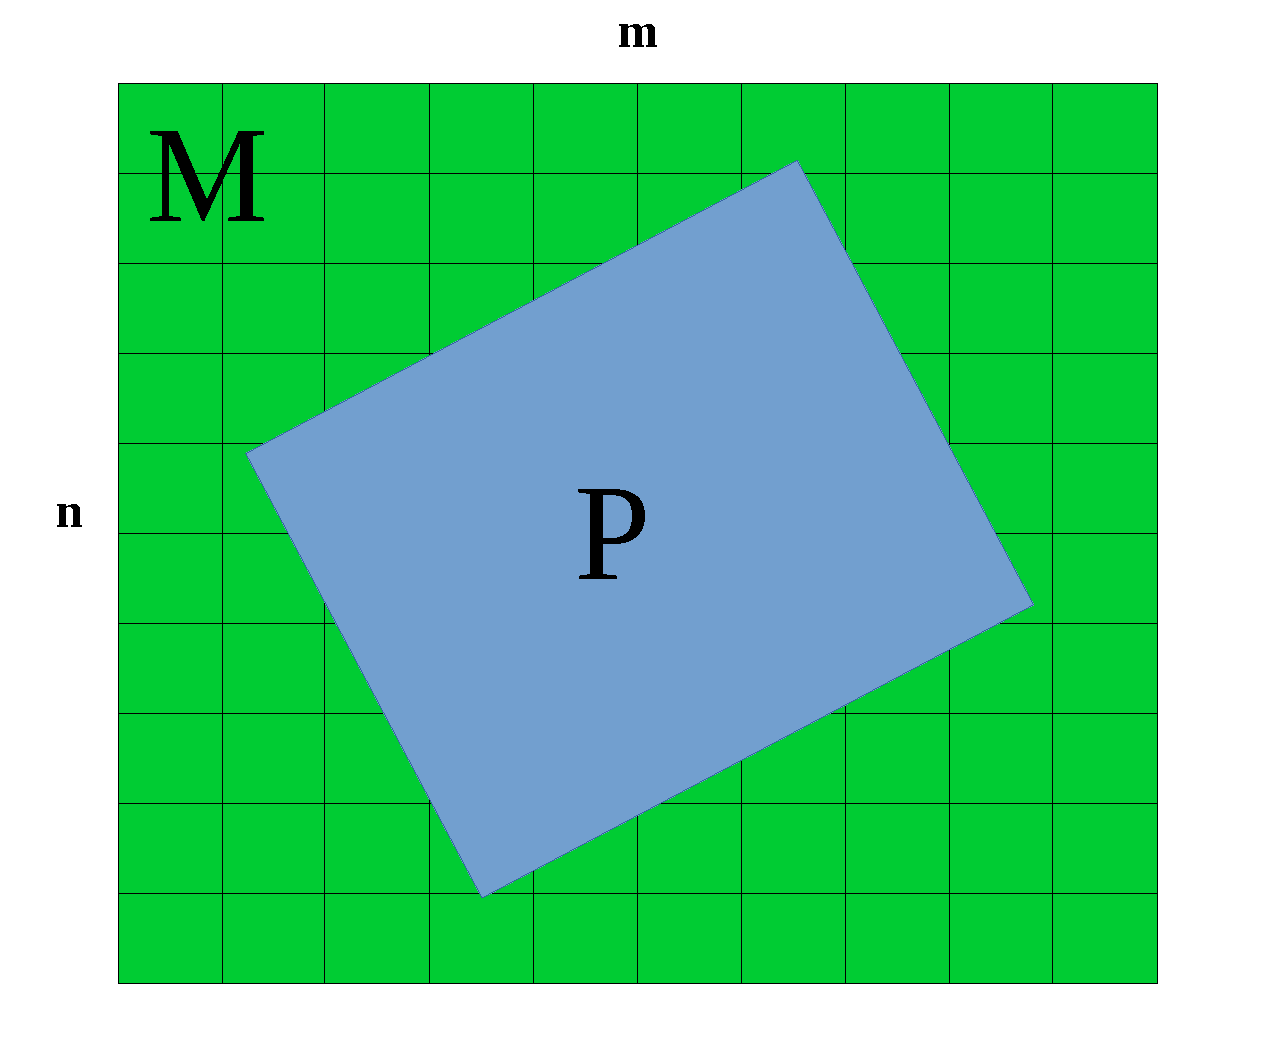
\includegraphics[ clip, scale=0.5]{mandf}}
	\centering
	\caption{blah}
	\label{fig:matrix_m}
\end{figure}
Załóżmy, że $p(x,y)$ jest funkcją mówiącą o tym czy punkt o współrzędnych $(x, y)$ znajduje się wewnątrz $P$. Jeśli $p = 0$ punkt należy do $P$, w przeciwnym wypadku $p=1$. Zraszacz jest definiowany jako okrąg reprezentowany przez promień $r_{i}$, współrzędne środka $(x_i, y_i)$ oraz konkretny model $t_{i}$. Środek każdego zraszacza musi zawierać się w $P$, czyli $p(x_{i}, y_{i}) = 0$.\\
Kwadrat o współrzędnych $(x,y)$ jest nawodniony jeśli znajduje się w zasięgu zraszacza. Jest to wyrażone następującą funkcją:
\begin{equation}
	is\_irr(x, y, s_{i}) = \begin{cases}
							1,& \text{jeśli } (x - x_{i})^{2} + (y - y_{i})^2 \leq r_{i}^{2}\\
							0,& w.p.p
						  \end{cases}
\end{equation}
, gdzie $x$ oraz $y$ oznaczają współrzędne środka kwadratu; $x_{i}, y_{i}$ oznaczają współrzędne zraszacza; $r_{i}$ jest liczba wyrażającą zasięg zraszacza.\\\\
Załóżmy, że $S$ jest zbiorem rozmieszczonych zraszaczy. Wtedy dany kwadrat jest nawodniony jeśli znajduje się w zasięgu przynajmniej jednego zraszacza ze zbioru $S$:
\begin{equation}
	irr(x, y, S) = \begin{cases}
				   	1,& \text{jeśli } \sum_{i=1}^{S} is\_irr(x,y,s_{i}) > 0 \\
				   	0,& w.p.p			   	
				   \end{cases}
\end{equation}
, gdzie $s$ jest konkretnym zraszaczem ze zbioru $S$.\\\\
Generalnie poprzez stopień nawodnienia danego obszaru rozumie się różnicę pomiędzy liczbą wszystkich elementów macierzy $M$ należących do $P$, a liczbą nawodnionych elementów tej macierzy należących do $P$:
\begin{equation}\label{eq:simple_f1}
	F_{0}(S) = \sum_{m=1}^{M}\sum_{n=1}^{N} p(m,n) \cdot (1 - irr(m,n,S))
\end{equation}

Im wartość funkcji $F_{0}$ jest mniejsza tym mniej jest obszarów nienawodnionych, a więc rozwiązanie jest lepsze. $F_{0} = $ jest rozwiązaniem idealnym z perspektywy kryterium nawodnienia.\\\\
Jak zostało wspomniane w poprzednich rozdziałach zaimplementowane algorytmy oceniają stopień nawodnienia obszaru na dwa sposoby w zależności od tego czy wybrana jest opcja minimalizacji nawodnienia poza wskazanym obszarem. Jeśli minimalizacja jest wyłączona do obliczeń używana jest prosta funkcja opisana powyżej \eqref{eq:simple_f1}. Bardziej szczegółowe rozwinięcie funkcji przewiduje wprowadzenie kary za naruszenie ograniczeń:

\begin{equation}
\begin{split}
	F_{1}(S) = \sum_{m=1}^{M}\sum_{n=1}^{N} p(m,n) \cdot (1 - irr(m,n,S)) \\ + 
	\alpha \cdot \bigg{[}\dfrac{\sum_{m=1}^{M}\sum_{n=1}^{N} (1 - p(m,n)) \cdot irr(m,n,S) \cdot 100}{\sum_{m=1}^{M}\sum_{n=1}^{N} p(m,n)} \\ + \dfrac{\sum_{m=1}^{M}\sum_{n=1}^{N} p(m,n) \cdot ovrirr(m,n,S) \cdot 100}{\sum_{m=1}^{M}\sum_{n=1}^{N} p(m,n)}\bigg{]}
\end{split}
\end{equation}
, gdzie $\alpha$ jest zmienną określającą to czy na funkcję celu wpływa minimalizacja nawodnienia poza wskazanym obszarem. Zmienna $\alpha$ może przyjmować wartość 0 lub 1. Jeśli $\alpha=1$ minimalizacja jest brana pod uwagę; $ovrirr(m,n,S)$ jest funkcją mówiącą czy dany obszar został nadmiernie nawodniony \eqref{eq:is_overirrigated_func}.
\begin{equation}\label{eq:is_overirrigated_func}
	ovrirr(x,y,S) = \begin{cases}
				1,& \text{jeśli } \sum_{i=1}^{S} is\_irr(x,y,s_{i}) > 1 \\
				0,& w.p.p
			   \end{cases}
\end{equation}
\\Jak zostało wspomniane wcześniej, każdy rozmieszczony zraszacz charakteryzowany jest przez konkretny model. Załóżmy, że $C(t_{i})$ jest funkcją zwracającą cenę rynkową dla danego modelu $t_i$. Wtedy całkowity koszt konkretnego rozwiązania wynosi:
\begin{equation}
	F_{2}(S) = \sum_{i=1}^{S} C(t_{i})
\end{equation}\\
Podsumowując celem zadania jest rozwiazanie następującego problemu optymalizacyjnego:

\begin{equation}
	\begin{split}
		min \text{  } & 	F_{1}(S) = \sum_{m=1}^{M}\sum_{n=1}^{N} p(m,n) \cdot (1 - irr(m,n,S)) \\ +& 
		\alpha \cdot \bigg{[}\dfrac{\sum_{m=1}^{M}\sum_{n=1}^{N} (1 - p(m,n)) \cdot irr(m,n,S) \cdot 100}{\sum_{m=1}^{M}\sum_{n=1}^{N} p(m,n)} \\ +& \dfrac{\sum_{m=1}^{M}\sum_{n=1}^{N} p(m,n) \cdot ovrirr(m,n,S) \cdot 100}{\sum_{m=1}^{M}\sum_{n=1}^{N} p(m,n)}\bigg{]}\\\\
		min \text{  }&	F_{2}(S) = \sum_{i=1}^{S} C(t_{i})
	\end{split}
\end{equation}

\subsection{Porównanie algorytmów genetycznych}
\subsubsection{Plan badań}
Złożoność oceny algorytmów służących do optymalizacji wielokryterialnej jest znacznie większa niż tej dla algorytmów rozwiązujących problemy obejmujące jedno kryterium. Wynika tak z samej definicji rozwiązania problemu wielokryterialnego, która wyjaśniona została wcześniej. Oceniając rozwiązanie takiego problemu należy wziąć pod uwagę następujące składowe:
\begin{itemize}
	\item Dystans znalezionego niezdominowanego zbioru rozwiązań od prawdziwego zbioru Pareto
	\item Równomierny rozkład znalezionych rozwiązań
	\item Długość przedziału pokrytego przez znalezione rozwiązania
	\item Czas wykonania algorytmu\\
\end{itemize}
Na potrzeby analizy i oceny dwóch zaproponowanych algorytmów wybrane zostały cztery metryki:
\begin{enumerate}
	\item \textit{Współczynnik błędu (ER):} wskazuje procent rozwiązań, które nie należą do prawdziwego zbioru Pareto.
	\begin{equation}
		ER = \dfrac{\sum_{i=1}^{n} e_{i}}{n}
	\end{equation}
	Gdzie $n$ jest liczbą znalezionych niezdominowanych rozwiązań; $e_{i}$ zmienną określającą czy dane rozwiązanie znajduje się w prawdziwym zbiorze Pareto. Jeśli $e_{i} = 0$ rozwiązanie znajduje się w prawdziwym zbiorze Pareto, w przeciwnym razie $e_{i} = 1$. $ER = 0$ oznacza idealne rozwiązanie.\\
	\item \textit{Równomierny rozkład (SP):} metoda mierząca wariancję dystansu sąsiadujących rozwiązań znajdujących się na znalezionym froncie Pareto.
	\begin{equation}
		SP = \sqrt{\dfrac{1}{n-1}\sum_{i=1}^{n}{(\overline{d} - d_{i})}^{2}}
	\end{equation}
	Gdzie $n$ jest liczbą znalezionych niezdominowanych rozwiązań; $d_{i}$ oznacza dystans Euklidesowy pomiędzy danym rozwiązaniem, a jego najbliższym sąsiadem; $\overline{d}$ jest wartością oznaczającą średni dystans pomiędzy rozwiązaniami. Wartość $SP = 0$ oznacza, że znalezione rozwiązania są rozłożone równomiernie.\\
	\item \textit{Jakość ogólna (DG):}  wskazuje jak daleko od prawdziwego zbioru Pareto znajduje się zbiór znalezionych niezdominowanych rozwiązań. Miara zdefiniowana w następujący sposób:
	\begin{equation}
		DG = \dfrac{\sqrt{\sum_{i=1}^{n} d_{i}^{2}}}{n}
	\end{equation}
	Gdzie $n$ oznacza liczbę znalezionych niezdominowanych rozwiązań; $d_{i}$ jest dystansem Euklidesowym pomiędzy danym rozwiązaniem, a najbliższym rozwiązaniem należącym do prawdziwego frontu Pareto. Wartość $DG = 0$ oznacza, że wszystkie znalezione rozwiązania leżą na prawdziwym froncie Pareto.\\
	\item \textit{Długość frontu (FE):} metoda wskazująca jak duży obszar jest pokryty przez znalezione niezdominowane rozwiązania.
	\begin{equation}
		FE = \sum_{k=1}^{K} \max_{i, j!=i} \sqrt{(f_{i}^{k} - f_{j}^{k})^{2}}
	\end{equation}
	Gdzie $K$ oznacza liczbę funkcji celu; $f_{i}^{k}$ jest wartością $i$-tego rozwiązania z perspektywy kryterium $k$.\\
\end{enumerate}
Aby skorzystać z powyższych metryk konieczne jest znalezienie prawdziwego frontu Pareto. Na potrzeby badań został on wygenerowany   poprzez wybranie niezdominowanych rozwiązań ze skumulowanej puli rozwiązań powstałej na wskutek uruchomienia symulacji 10 razy dla każdego algorytmu. Rezultaty każdej symulacji były dodawane do puli po czym zredukowane do rozwiązań niezdominowanych.\\
Dla badań przygotowanych zostało 6 przypadków testowych. Zostały one podzielone ze względu na wielkość obszaru mającego zostać nawodniony oraz tego czy algorytm ma minimalizować nawadnianie poza zaznaczonym obszarem. Kształt wybranych obszarów został dobrany tak, aby jak najlepiej wizualizować wpływ ograniczeń na działanie algorytmów.

\begin{table}[]
\centering
\caption{Przypadki testowe}
\label{my-label}
\begin{tabular}{|l|l|}
\hline
Wielkość & Obszar \\ \hline
Mały & 1 \\ \hline
Średni & 2 \\ \hline
Duży & 3 \\ \hline
\end{tabular}
\end{table}

\subsubsection{Rezultaty badań}
\subsubsection{Podsumowanie badań}

\chapter{Podsumowanie}

\begin{mydef}
\textbf{Definicja} - pierwsza
\end{mydef}




 \clearpage
\appendix
\chapter{Appendix 1}


\clearpage
\pagestyle{plain}
\listofmyfigure
\listofmyequations
\listofmyalgorithm
\clearpage

%\bibliographystyle{apalike}%Used BibTeX style is unsrt

\bibliographystyle{iisthesis}
\bibliography{bibliography}

\end{document}

